% Header define
\documentclass[compress]{beamer}
\usepackage[utf8]{inputenc}
\usepackage{textpos} % package for the positioning
\usepackage{listings}

\usetheme{Warsaw}
\title[Memory analysis and password manager]{
  Memory analysis and password manager\\
  All your passwords are belong to us
}
\author[y0ug - Hugo Caron]{
\includegraphics[width=4cm,keepaspectratio]{logo}\\y0ug - Hugo Caron}
\institute{itrust.lu}
\date{9 June 2012}
%\logo{
\includegraphics[height=0.5cm]{logotype}} 

%\definecolor{grey}{HTML}{e6e6e6} % vert moyen
%\setbeamercolor{background canvas}{bg=grey}

\definecolor{green}{HTML}{01d300} % matrix
\definecolor{yellow}{HTML}{e0dF00} % matrix
%\setbeamercolor{frametitle}{bg=green!85!yellow}
\setbeamercolor{frametitle}{bg=black}
\setbeamercolor{subsection in head/foot}{bg=black}


\setbeamertemplate{blocks}[rounded][shadow=false]


%\setbeamertemplate{headline}{\vskip2pt}  % remove headline
%\documentclass[compress]{beamer}
%\setbeamertemplate{headline}{}

\setbeamertemplate{title page}[default][colsep=-4bp,rounded=true,shadow=flase]
%\setbeamercolor{block title}{bg=green}
%\setbeamercolor{palette primary}{bg=green}
%\setbeamercolor{palette quaternary}{bg=green}

\addtobeamertemplate{frametitle}{}{%
\begin{textblock*}{50mm}(0.965\textwidth, -0.77cm)

\includegraphics[height=0.69cm,keepaspectratio]{logotype}
\end{textblock*}}

\begin{document}


% First slide title page
\begin{frame}
\titlepage
\end{frame}

% TOC
\begin{frame}{Plan}
  \tableofcontents[]
\end{frame} 

% Section presentation
\section{Presentation}
\begin{frame}[fragile]{Introduction}
We're going to explain how we manage to recover data 
from different password manager, by analysing two cases:
  \begin{itemize}
    \item PasswordKeeper with no protection against memory dump
    \item KeepessX where data are encrypted in memory
  \end{itemize}
\end{frame}

\begin{frame}{Tools}
To manage this task we used:
  \begin{itemize}
    \item Volatility and the module
      \begin{itemize}
        \item memdump
        \item procmemdump
        \item volshell
      \end{itemize}
    \item IDA (for KeepassX)
  \end{itemize}
\vspace{0.2in}
All our tests are done on memory dump of WinXP SP3 in VirtualBox
\end{frame}

% Section PasswordKeeper
\section{PasswordKeeper}
\subsection{Introduction}
\begin{frame}{Information}
  \begin{columns}[T]
    \begin{column}{.5\textwidth}
      \begin{block}{Description from official website}
"Password Keeper is a small utility
useful for storing your frequently
used passwords. Password
information can be stored,
edited and printed with this easy
to use program."\\
      \end{block}
    \end{column}
    \begin{column}{.5\textwidth}
      \begin{block}{User interface}
        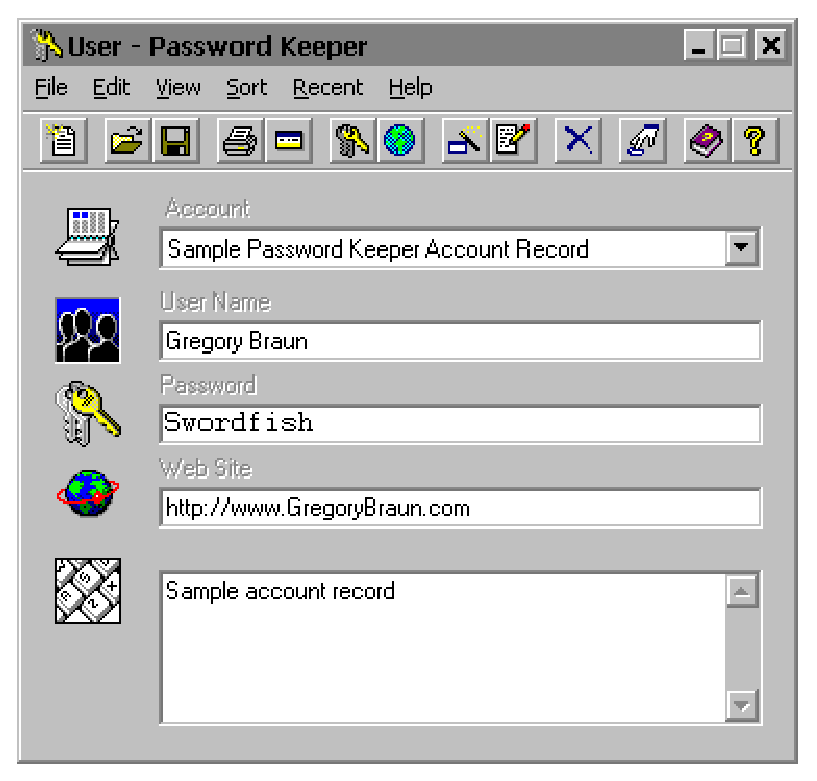
\includegraphics[width=\textwidth]{img/passwordkeepergui.eps}
      \end{block}
    \end{column}
  \end{columns}
\end{frame}

\begin{frame}{Dump creation}
In the next slides we work on a system memory dump with a running 
process of Password Keeper. \\
\vspace{0.2in}
To facilitate the password container
contains this following data:
  \begin{itemize}
    \item Account: Foo
    \item Username: Baz
    \item Password: rqNBikbt
    \item URL: http://www.bar.baz
    \item Comment: SuperComment
  \end{itemize}
\end{frame}

\subsection{Exploitation}
\begin{frame}{Recover information}

  \setbeamertemplate{blocks}[rounded][shadow=false]
  \begin{block}{With volatilty we dump the PasswordKeeper processes}
    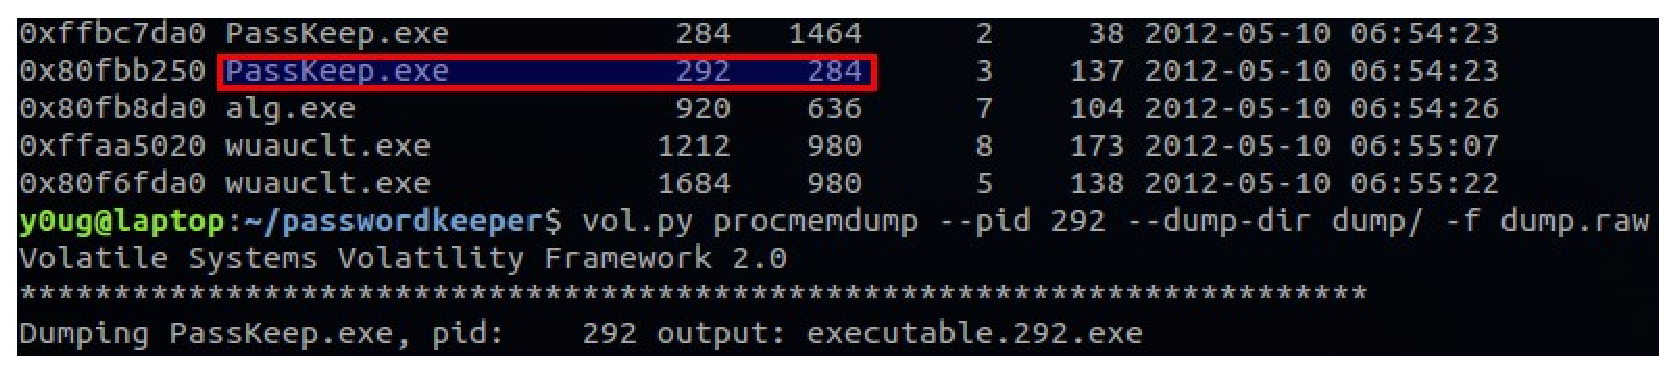
\includegraphics[width=\textwidth]{img/passwordkeeper_dump.eps}
  \end{block}

  \setbeamertemplate{blocks}[rounded][shadow=false]
  \begin{block}{And strings our password on it}
    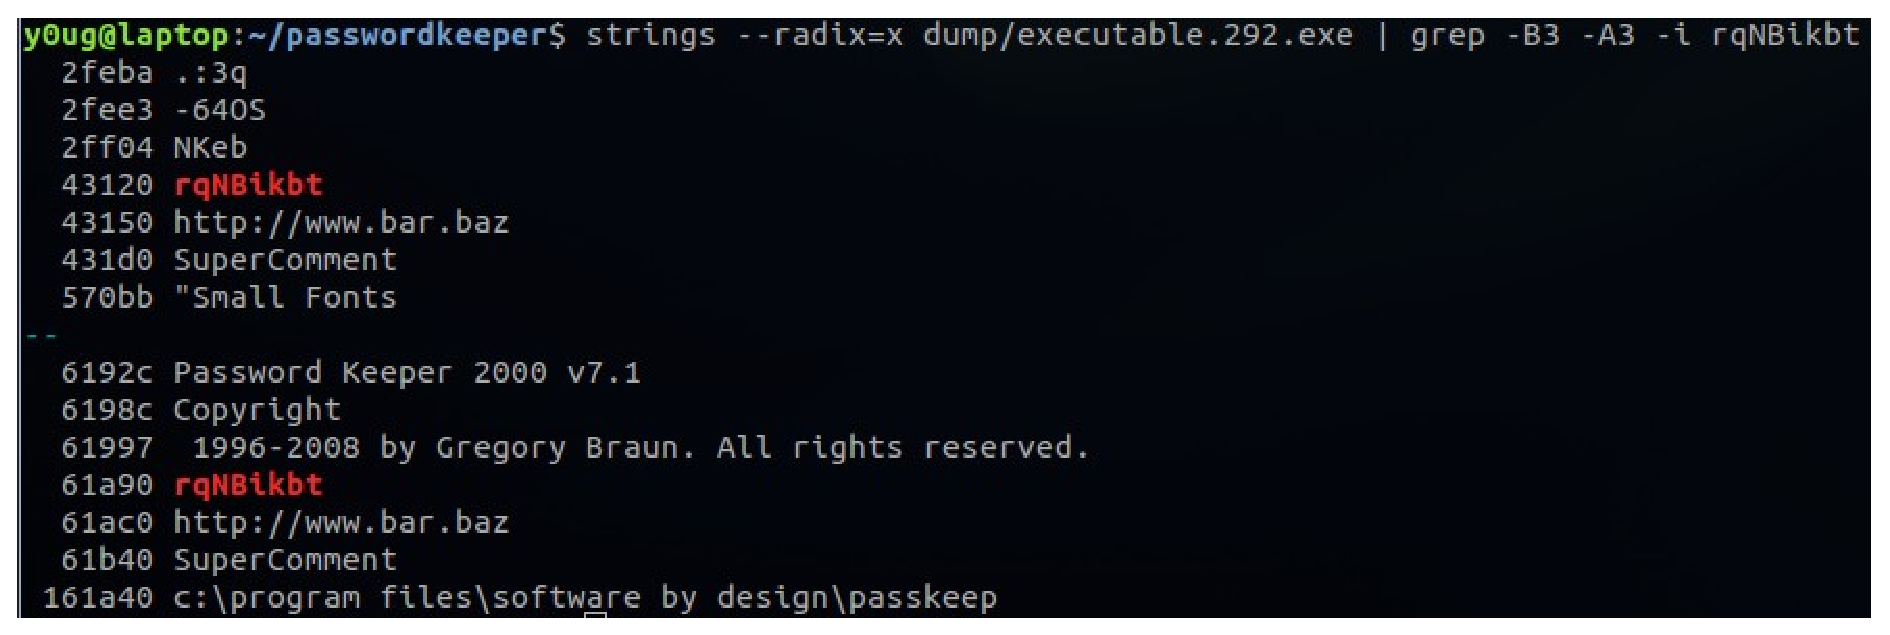
\includegraphics[width=\textwidth]{img/passwordkeeper_strings.eps}
  \end{block}

\end{frame}

\begin{frame}{Extracting data structure}
      \setbeamertemplate{blocks}[rounded][shadow=false]
      \begin{block}{Information}
Data are in clear text, good news.\\
With more investigation we manage to
recover:
        \begin{itemize}
          \item The structure
          \item A signature to match the position in dump
        \end{itemize}
      \end{block}

  \begin{columns}[T]
    \begin{column}{.4\textwidth}

      \setbeamertemplate{blocks}[rounded][shadow=false]
      \begin{block}{structure}
        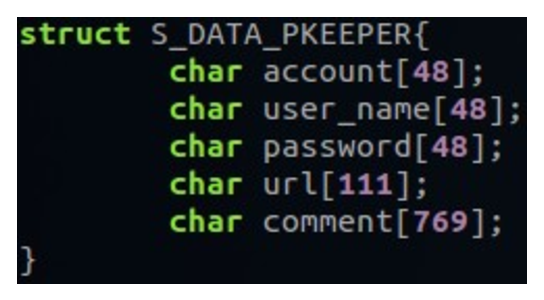
\includegraphics[width=\textwidth]{img/passwordkeeper_struct.eps}
      \end{block}
    \end{column}
    \begin{column}{.6\textwidth}

      \setbeamertemplate{blocks}[rounded][shadow=false]
      \begin{block}{Signature}
        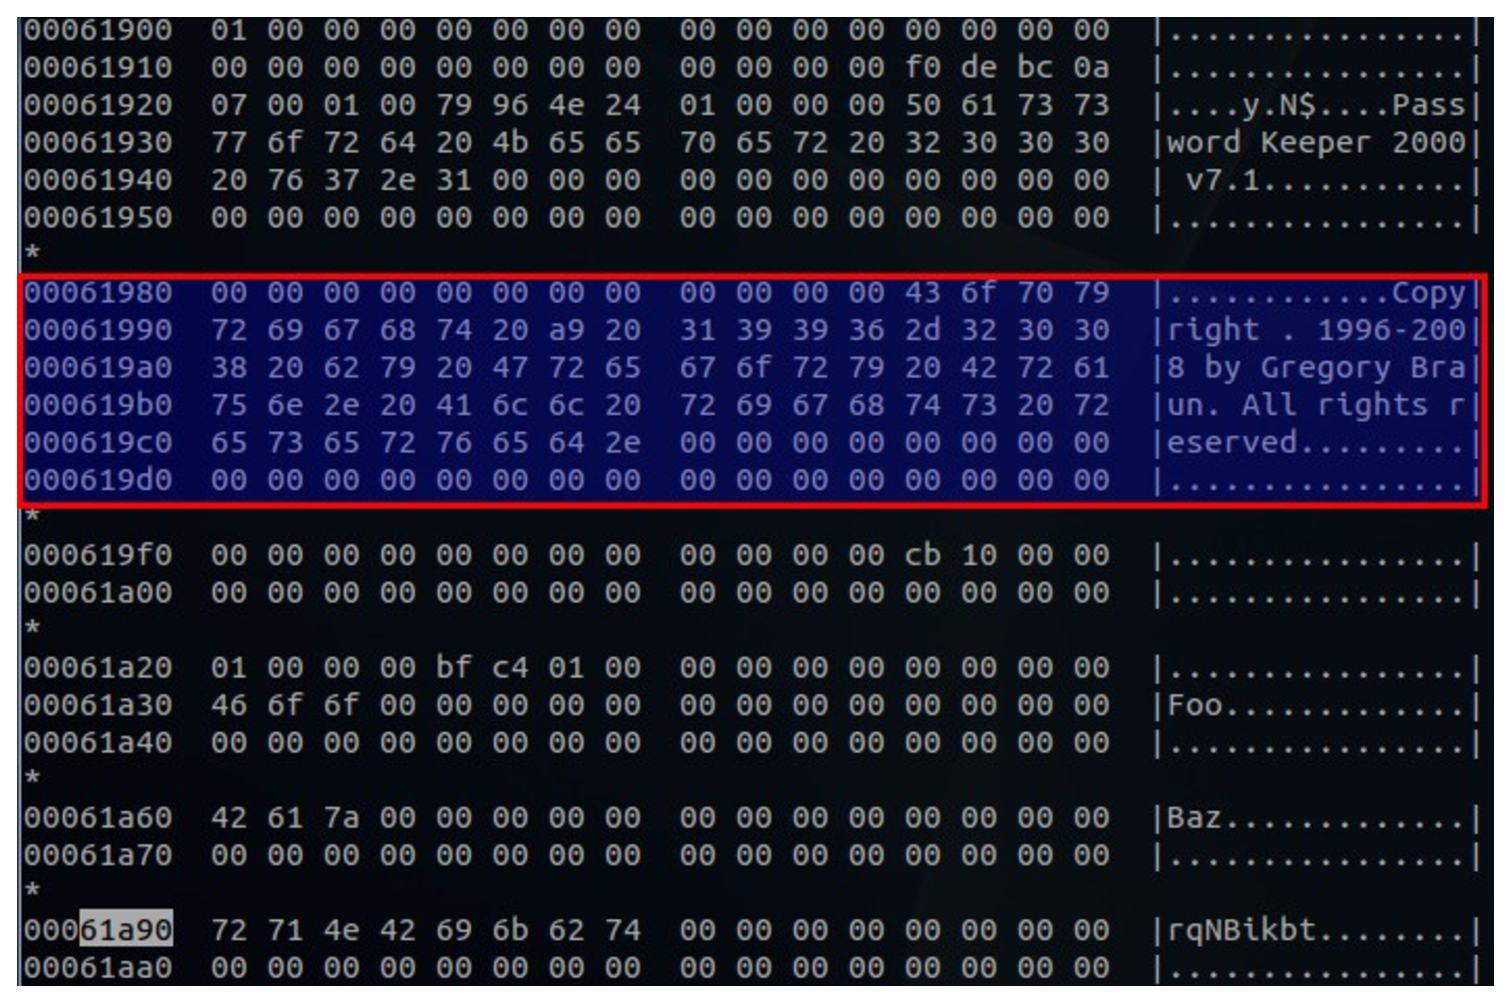
\includegraphics[scale=0.2]{img/passwordkeeper_sign.eps}
      \end{block}
    \end{column}
  \end{columns}

\end{frame}

\begin{frame}{Script}
With this information we wrote a ruby script to extract automatically all entry:
\end{frame}

\section{KeepassX}
\subsection{Introduction}
\begin{frame}{Introduction}
  \begin{itemize}
    \item Is a cross platform password manager.
    \item On the official website no specifics information about protection against memory dump
    \item It uses AES cbc to encrypt the file container
    \item Advantage we've the code
  \end{itemize}
  \begin{center}
    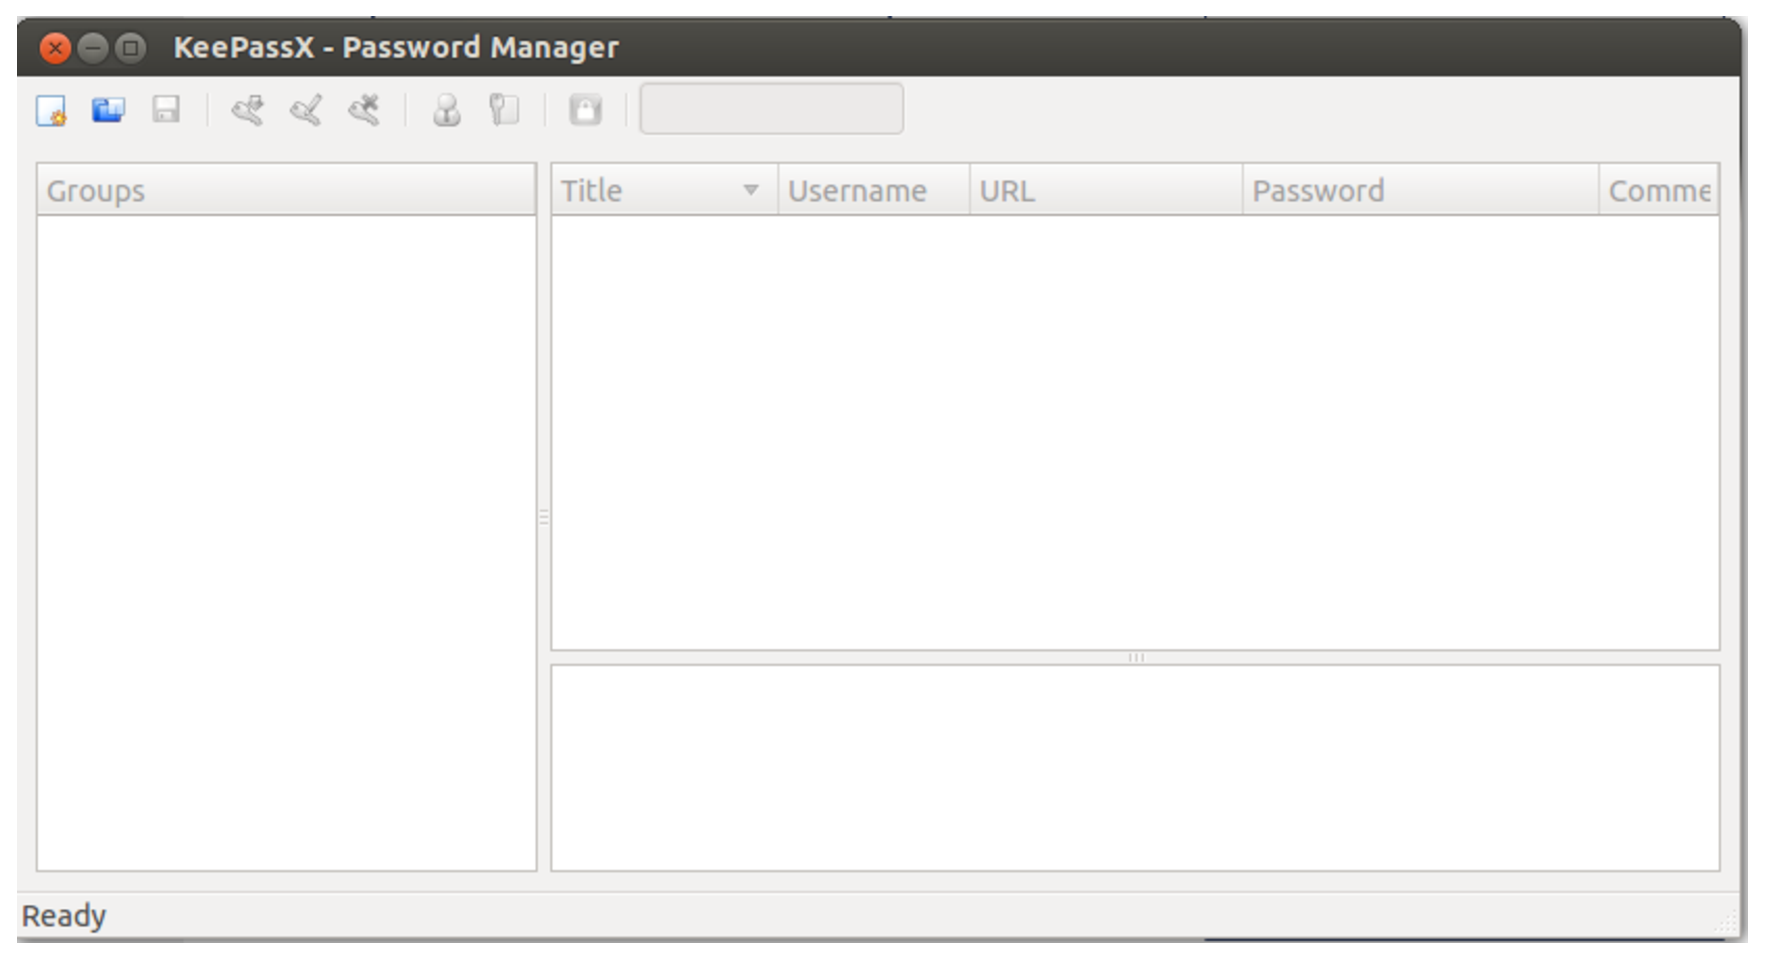
\includegraphics[scale=0.2]{img/keypass.eps}
  \end{center}
\end{frame}

\begin{frame}{Introduction}
  We do some classic check with strings to try to recover data in a memory dump of the process:
  \begin{itemize}
    \item No conclusive results
    \item We've the source code so we use it
  \end{itemize}
  \vspace{0.1in}
  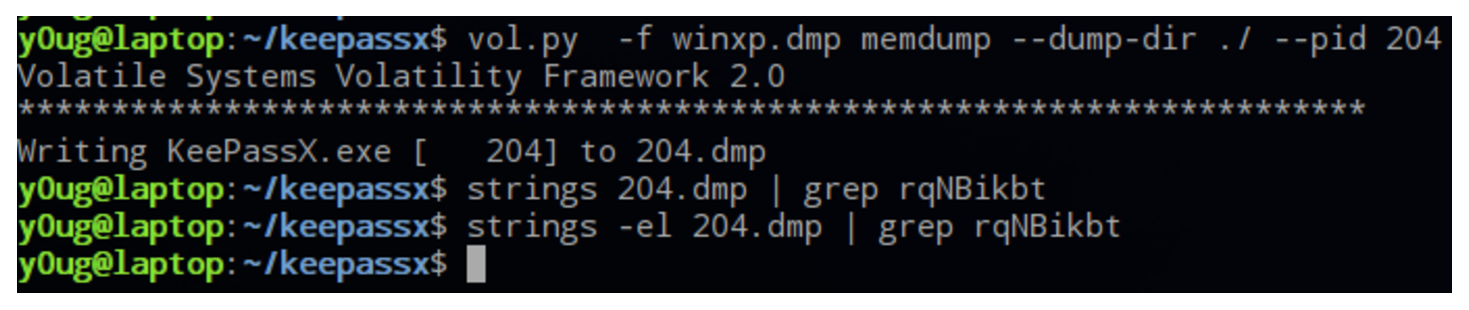
\includegraphics[scale=0.4]{img/keypass_strings_test.eps}
\end{frame}

\subsection{How it works?}
\begin{frame}{Data loading}
  With the source code we understand how it loads data from the container in memory:
  \begin{itemize}
    \item Load the file in memory
    \item Recover information need to decrypt the file like EncryptionIV, ContentHash, FinalRandomSeed etc..
    \item Check magic, version and flag
    \item Compute a SHA256 composed of FinalRandomSeed + Masterkey
    \item Transform the SHA256 of the masterkey
    \item Decrypt the container with AES CBC, the EncryptionIV and the last compute hash
    \item Check if ContentHash match the decrypt data
  \end{itemize}
\end{frame}

\begin{frame}[fragile]{Memory protection}
  \begin{columns}[T]
    \begin{column}{.4\textwidth}
      %\setbeamertemplate{blocks}[rounded][shadow=false]
      %\begin{block}{Information}
  We know that the MasterKey are in \verb|SecData RawMasterKey|\\
  \vspace{0.1in}
  \verb|SecData| is a class that secure data in memory, when the software don't need it, it locks the data (encrypt data with a cutsom RC4)\\
  \vspace{0.1in}
  The variable can be represented like this:
      %\end{block}
    \end{column}
    \begin{column}{.6\textwidth}
  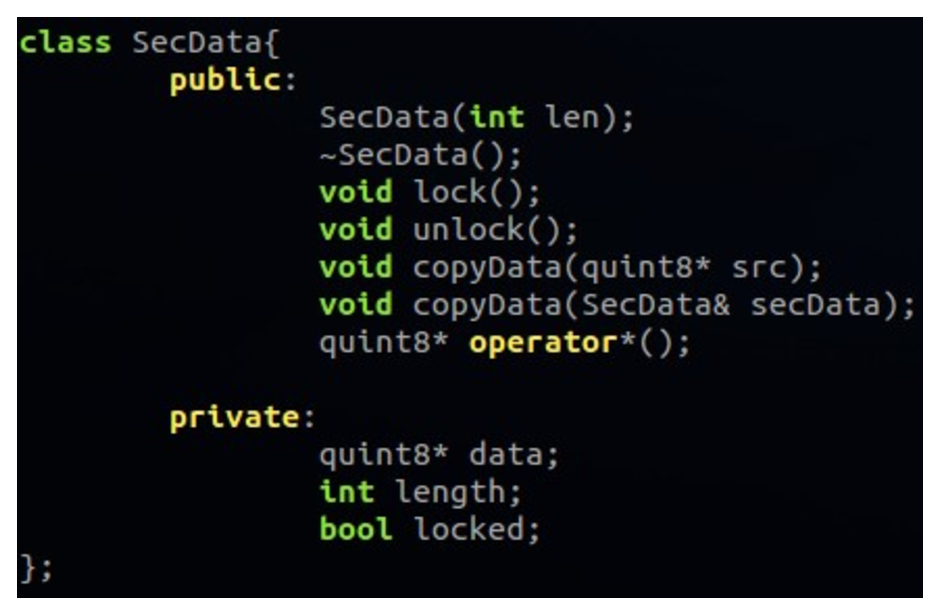
\includegraphics[scale=0.35]{img/keypass_secdata.eps}
     \begin{block}{Memory representation}
  \begin{lstlisting}
|  pdata|length|  locked|
|XXXXXXX|    20|00000001|

Length = 32 (SH256 len)
Locked = 1  (Lock flag)
  \end{lstlisting}
      \end{block}
    \end{column}
  \end{columns}
\end{frame}

\begin{frame}[fragile]{RC4 key}
  \begin{columns}[T]
    \begin{column}{.5\textwidth}
  To encrypt data in memory it uses the same key for all data (in \verb|class SecString|)\\
  \verb|static quint8 *sessionkey;|\\
  \vspace{0.1in}
  Is a static variable, so it will be at same memory address in each dump.\\
  \vspace{0.1in}
  The algorithm used to encrypt data is modified RC4 version
  \vspace{0.1in}
    \end{column}
    \begin{column}{.5\textwidth}
  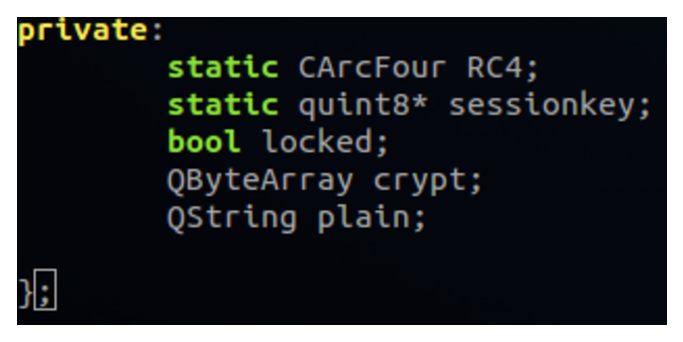
\includegraphics[scale=0.5]{img/keypass_secstring.eps}
    \end{column}
  \end{columns}
\end{frame}

\begin{frame}[fragile]{RC4 key}
  To recover the address of: \verb|static quint8* sessionkey| we use IDA with the targeted version of KeepassX.\\
  We've to look in \verb|SecString::generateSessionKey()|:\\
  \vspace{0.1in}
  \begin{center}
  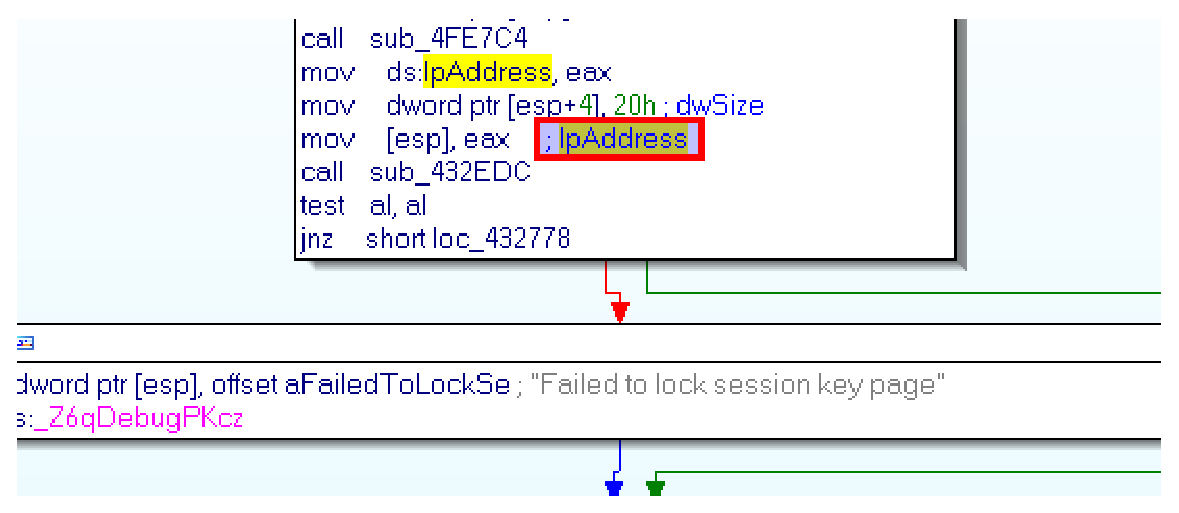
\includegraphics[scale=0.4]{img/keypass_ida_session}\\
  \vspace{0.1in}
  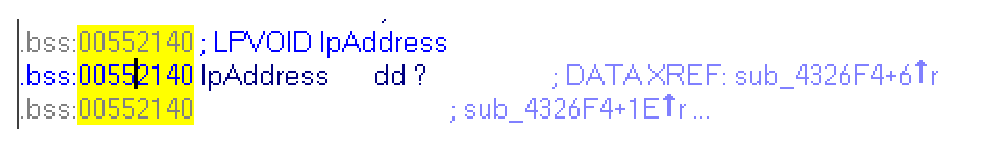
\includegraphics[scale=0.4]{img/keypass_ida_session_adr}\\
  \end{center}
  \vspace{0.1in}
  In our case the address is \verb|00552140h|\\
\end{frame}

\subsection{Summarize}
\begin{frame}[fragile]{Summarize}
  Summarize, we know:
  \begin{itemize}
    \item The file format of kdb
    \item The address of the RC4 key used to crypt the master key in memory
    \item Structure to seek to find the pointer to the encrpyted master key
    \item Algorithm to decrypt the container
  \end{itemize}
  \vspace{0.2in}
  So we've all information to recover data
\end{frame}

\subsection{Exploitation}
\begin{frame}{Recover address of encrypted master key}
  To recover the address of the encrypted master key we used a regex, on the memdump of the process.\\
  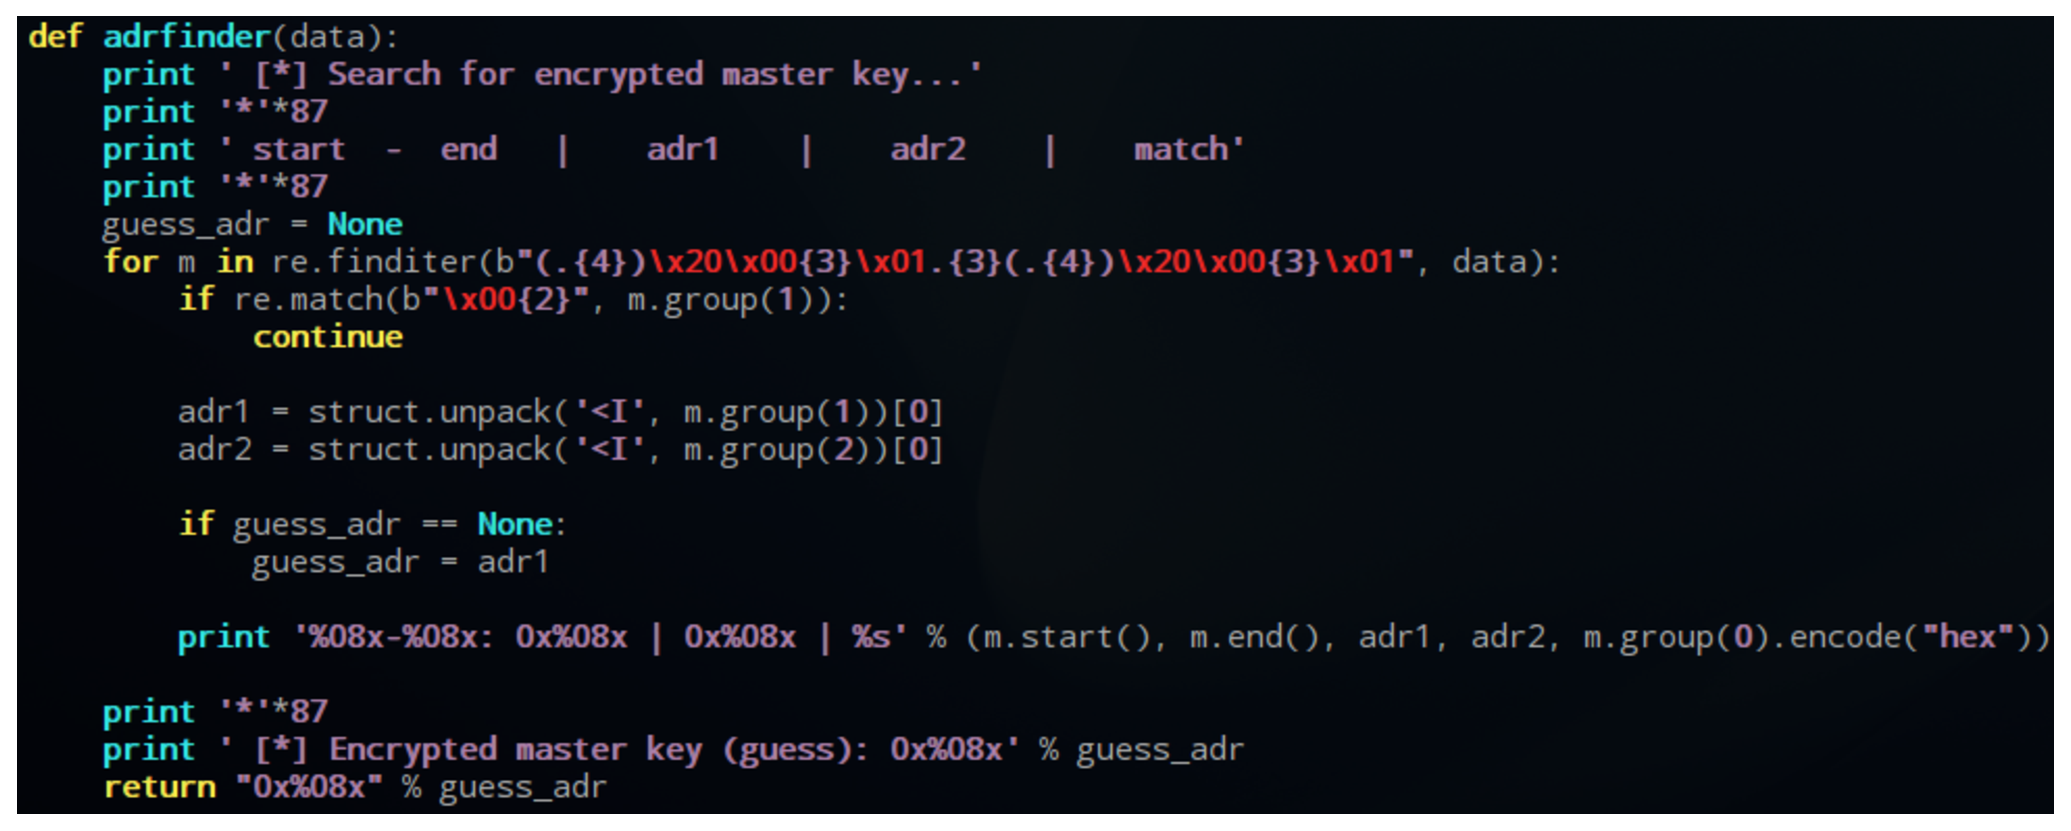
\includegraphics[scale=0.35]{img/keypass_adr_finder}\\
  The function take in input the memdump of the process, and return the first address that match the regex. The first is valid normally.
\end{frame}

\begin{frame}{Extract the encrypted master key}
  To extract the encrypted masterkey we used volatilty with the plugin volshell and the address found in the previous slides.\\
  \vspace{0.2in}
  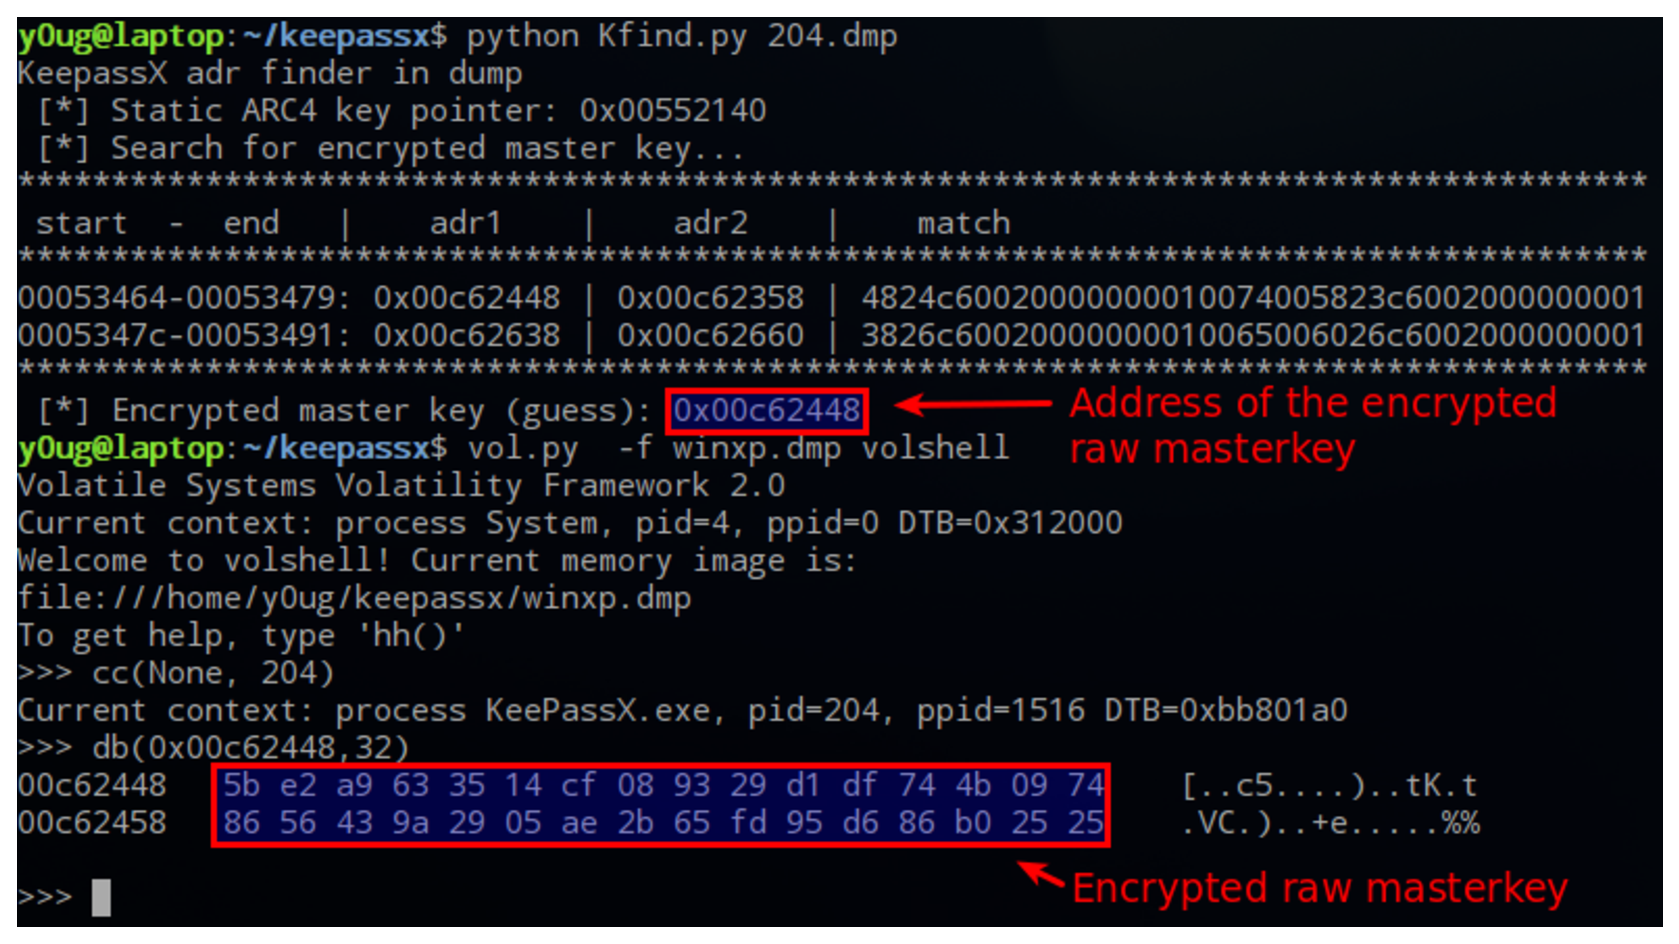
\includegraphics[scale=0.35]{img/keypass_volshell_masterkey}\\
\end{frame}

\begin{frame}{Extract the session key}
  To extract the session we used the same technique as above, with one more step to extract the value of the pointer founds with IDA.\\
  \vspace{0.2in}
  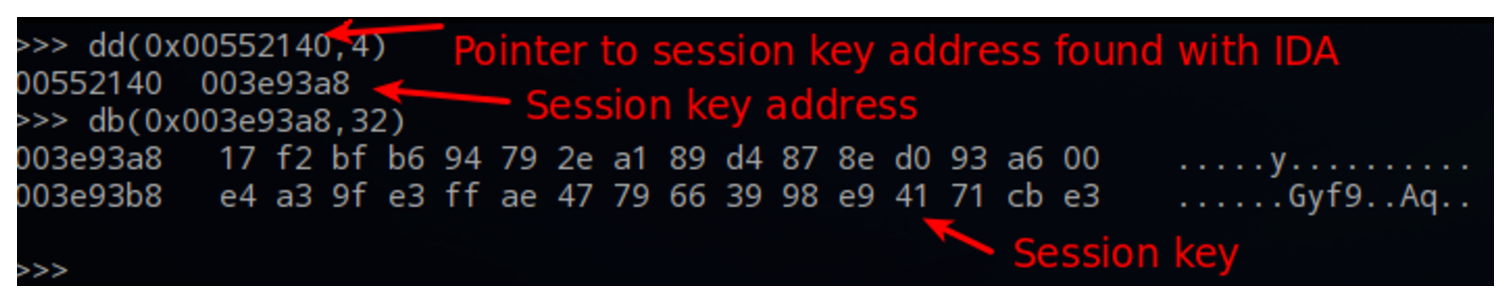
\includegraphics[scale=0.40]{img/keypass_volshell_sessionkey}\\
\end{frame}

\begin{frame}{Extract data from the container}
  We decrypt the masterkey and try to decrypt the password container by following the step define above.\\
  \vspace{0.2in}
  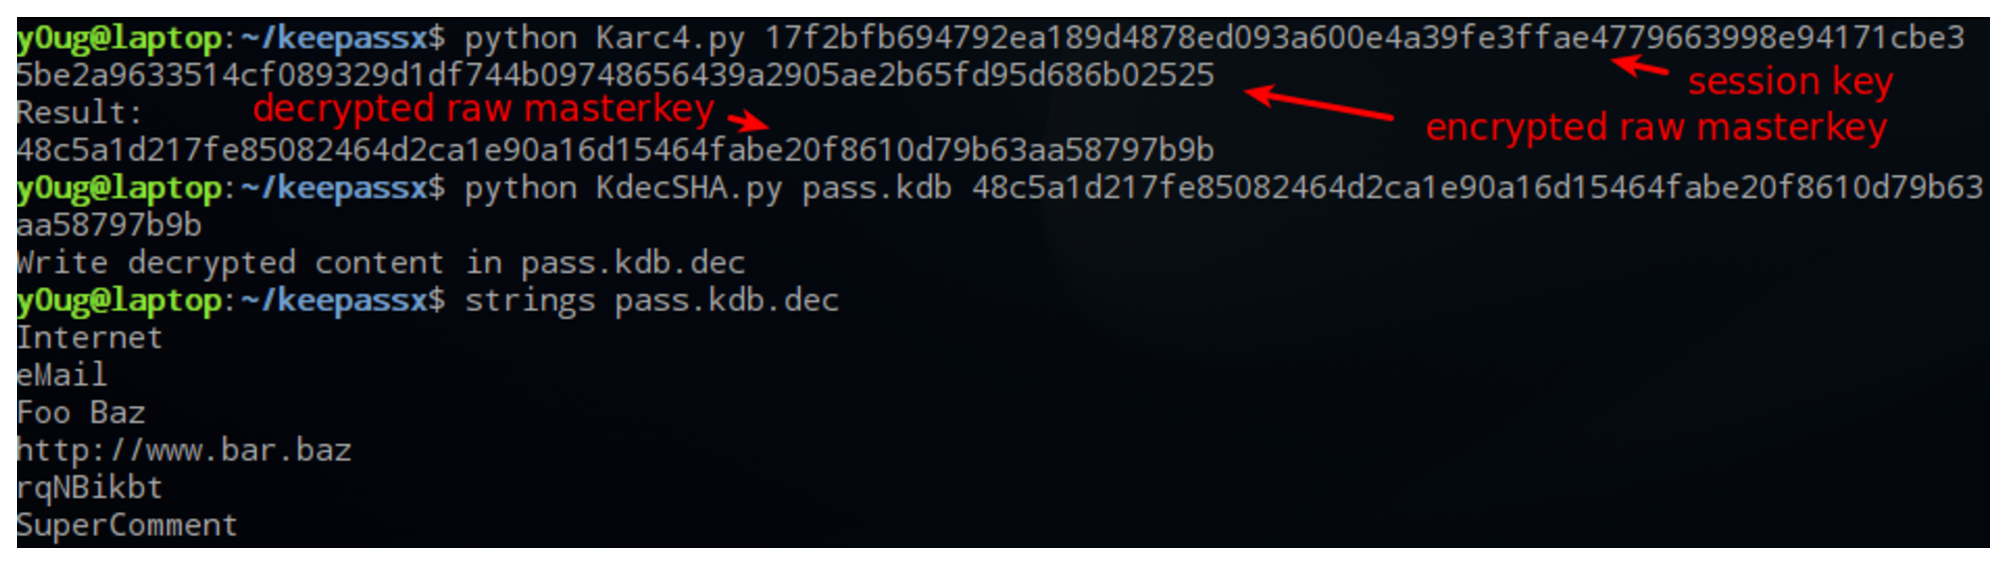
\includegraphics[scale=0.35]{img/keypass_recover_data}\\
\end{frame}

\subsection{Demo}
\begin{frame}{Demo}
  DEMO
\end{frame}

\section{Conclusion}
\begin{frame}{Conclusion}
  \begin{itemize}
    \item In this 2 cases we saw, the most current no protect at all and data encrypted in memory.
    \item We manage to prove that is possible to recover the container or the data from a a memory dump
    \item From a forensics point of view, this can help during investigation if the authorities have the idea to dump the memory before seizure.
    \item From an attacker point of view, this techniques can be apply too, with only a dump of the running process. It can be interesting to avoid for the attacker to wait with a key-logger that the target type the password.
  \end{itemize}
\end{frame}

\begin{frame}{Conclusion}
  \begin{center}
  Thank you for your attention.\\
  \vspace{0.2in}
  Any question? (or not)
\end{center}
\end{frame}

\end{document}
